\documentclass[12pt]{article}

\usepackage[utf8]{inputenc}

\usepackage[left=0.5in,right=0.5in,top=0.5in,bottom=0.5in]{geometry}

\usepackage[export]{adjustbox}
\usepackage{graphicx}
\graphicspath{ {/} }

\frenchspacing

\title{Beágyazott rendszerek szoftvertechnológiája HF - Specifikáció\vspace{-6ex}}

\date{}

\pagenumbering{gobble}

\begin{document}
\maketitle

\begin{Huge}
\begin{center}
\textbf{BATTLE CITY VERSUS}
\end{center}
\end{Huge}

\centering
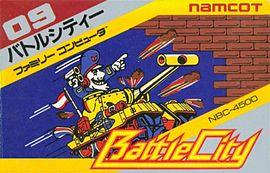
\includegraphics{Battle_City_NES_cover}


2D felülnézetes lövöldözős játék tankokkal, egy és többjátékos módban

\begin{itemize}
\item[] 14. Csoport:
\item[] \textbf{Kardos Bálint - ZI84PX} 
\item[] \textbf{Bauer Péter - FUHTUD}
\item[] \textbf{Murányi Péter - A74MW9}
\end{itemize}

\begin{itemize}

\item[] Játékmenet:

\begin{itemize}
\item[•] A játékos egy 2D grid-en tud mozogni négy irányba
\item[•] A tankkal egyes lövéseket tud leadni megadott maximális időközzel
\item[•] A pályán falak vannak elhelyezve melyek akadályt jelentenek a tankoknak és lövedékeknek
\item[•] A játékos nehézségi szinttől függően adott mennyiségű lövést tud elviselni mielőtt veszít
\end{itemize}

\item[] Játékmódok:

\begin{itemize}

\item[-] Egyjátékos:
\begin{itemize}
\item A játékos célja hogy minél több tankot kilőve minél magasabb pontszámot érjen el
\item Az ellenséges tankok egyesével jelennek meg a pályán véletlen helyeken
\item Az ellenséges tankok egy lövéstől megsemmisülnek
\item Az ellenséges tankok legrövidebb úton a játékos felé haladnak, ha rálátása van a játékosra megáll és lövéseket kezd el leadni
\item A lövések időköze és megállás és lövés közötti várakozás a nehézségi szinttől függ
\end{itemize}
\item[-] Többjátékos:
\begin{itemize}
\item Két játékos TCP kapcsolaton keresztül, egyik szerver másik kliens
\item A két játékosnak fix mennyiségű élete van, aki előbb kilövi a másikat az nyer
\end{itemize}

\end{itemize}

\end{itemize}

\end{document}